\section{Features}

(Should we present this information in a bullet list or in paragraphs?)

\begin{enumerate}

\item Map View - easy navigation and quick browsing

  \begin{itemize}

  \item Pan and zoom the sky map by dragging and scrolling

  \item Toggle and view specific catalog layers and multi-wavelength survey images

  \item Pop-ups over each source for basic information

  \item Powerful search tools - locate objects by name, association, or coordinate position

  \item Export and share a specific view of the sky map via PNG

  \end{itemize}


\item Catalog View - deeply investigate a specific source

  \begin{itemize}

  \item Search tool to find a source in its respective catalog by source name

  \item Basic info, extension info, spectral info, distance info

  \item Light curves, emission spectra (currently only for 3FGL catalog)

  \item References to which telescope detected the source and links to where our data came from

  \end{itemize}


\item Further analysis of our data with tools like Gammapy (generate specific plots, etc.)

\item Mention again that all data is openly available for download

\end{enumerate}

\begin{figure}[tb]
  \centerline{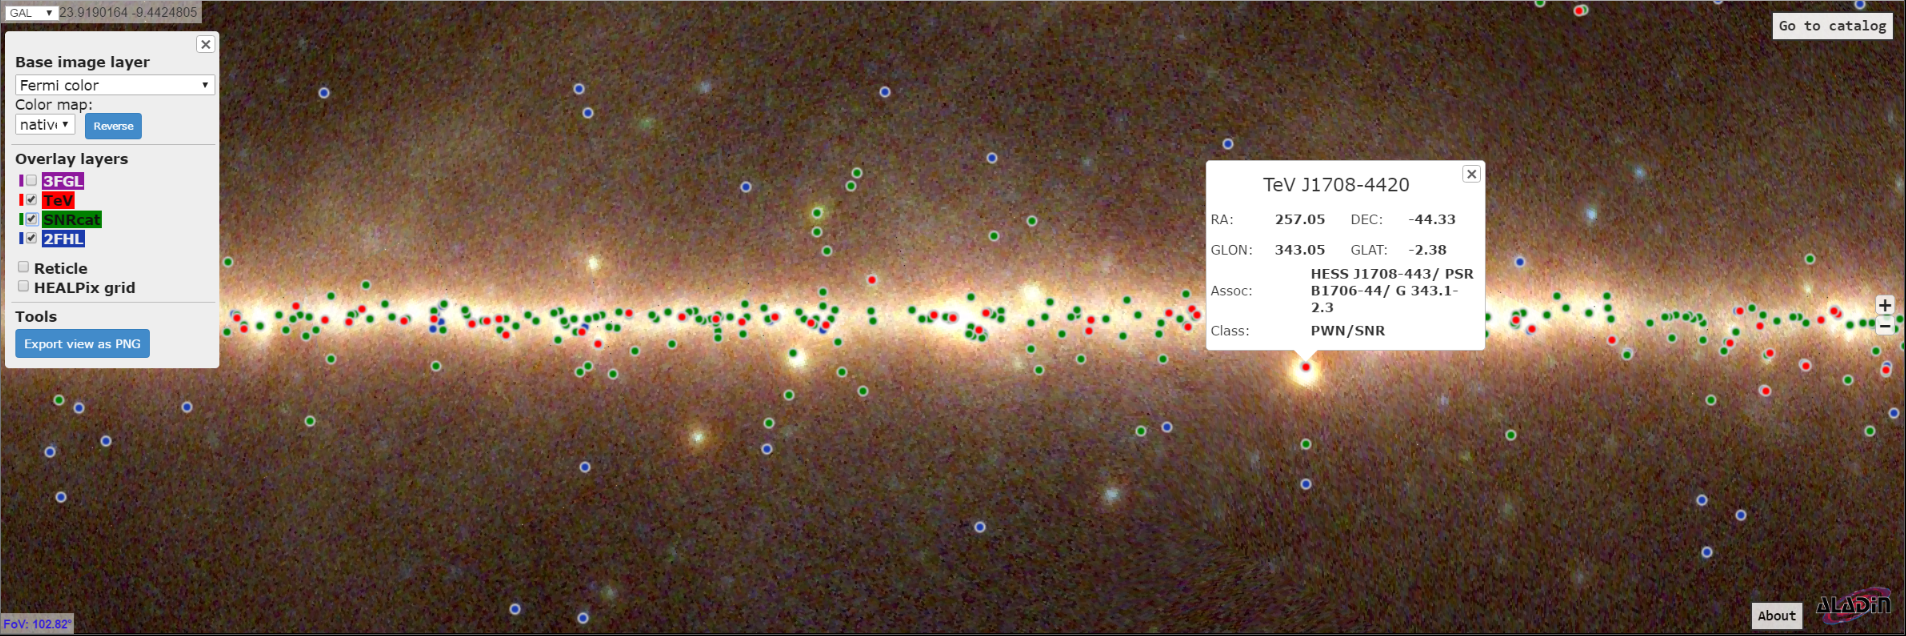
\includegraphics[width=\textwidth]{figures/mapview_wide}}
  \caption{Map View.}
\end{figure}

\begin{figure}[tb]
  \centerline{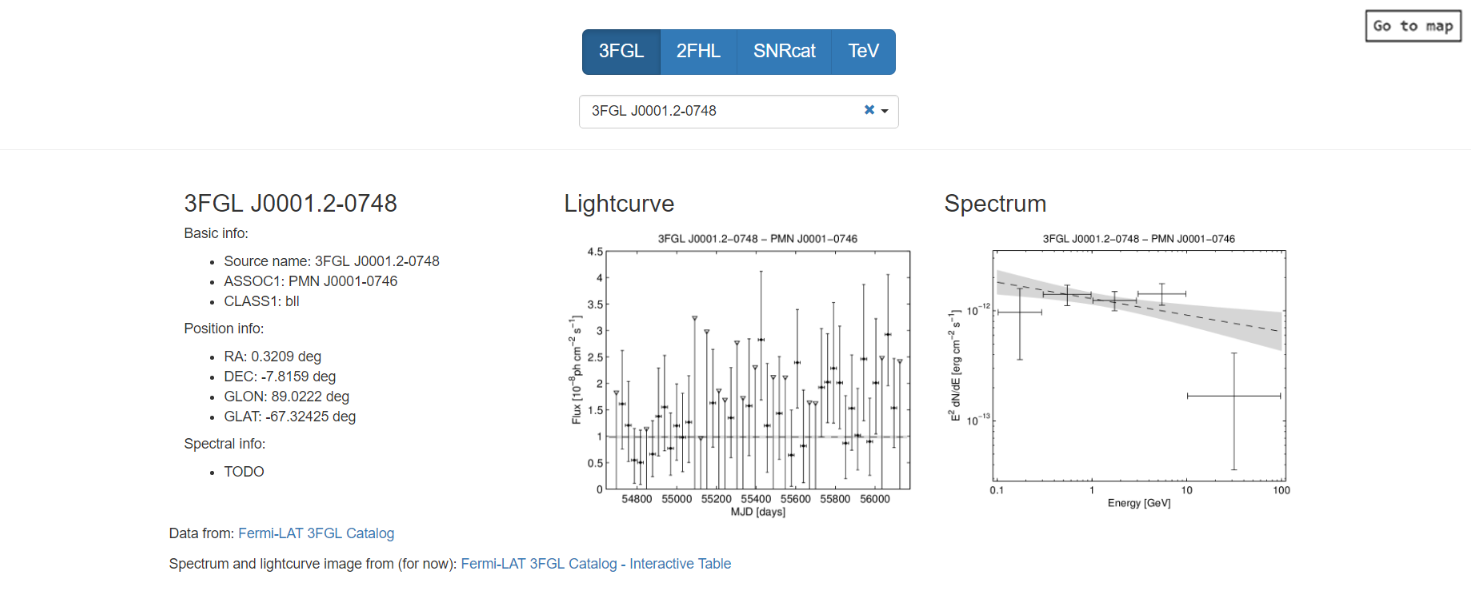
\includegraphics[width=\textwidth]{figures/catview_wide_zoom}}
  \caption{Catalog View.}
\end{figure}
